\documentclass[border=2pt]{standalone}
\usepackage{tikz}
\usetikzlibrary{quotes,angles}
\usepackage{amsmath}
\usepackage{amssymb}

\begin{document}

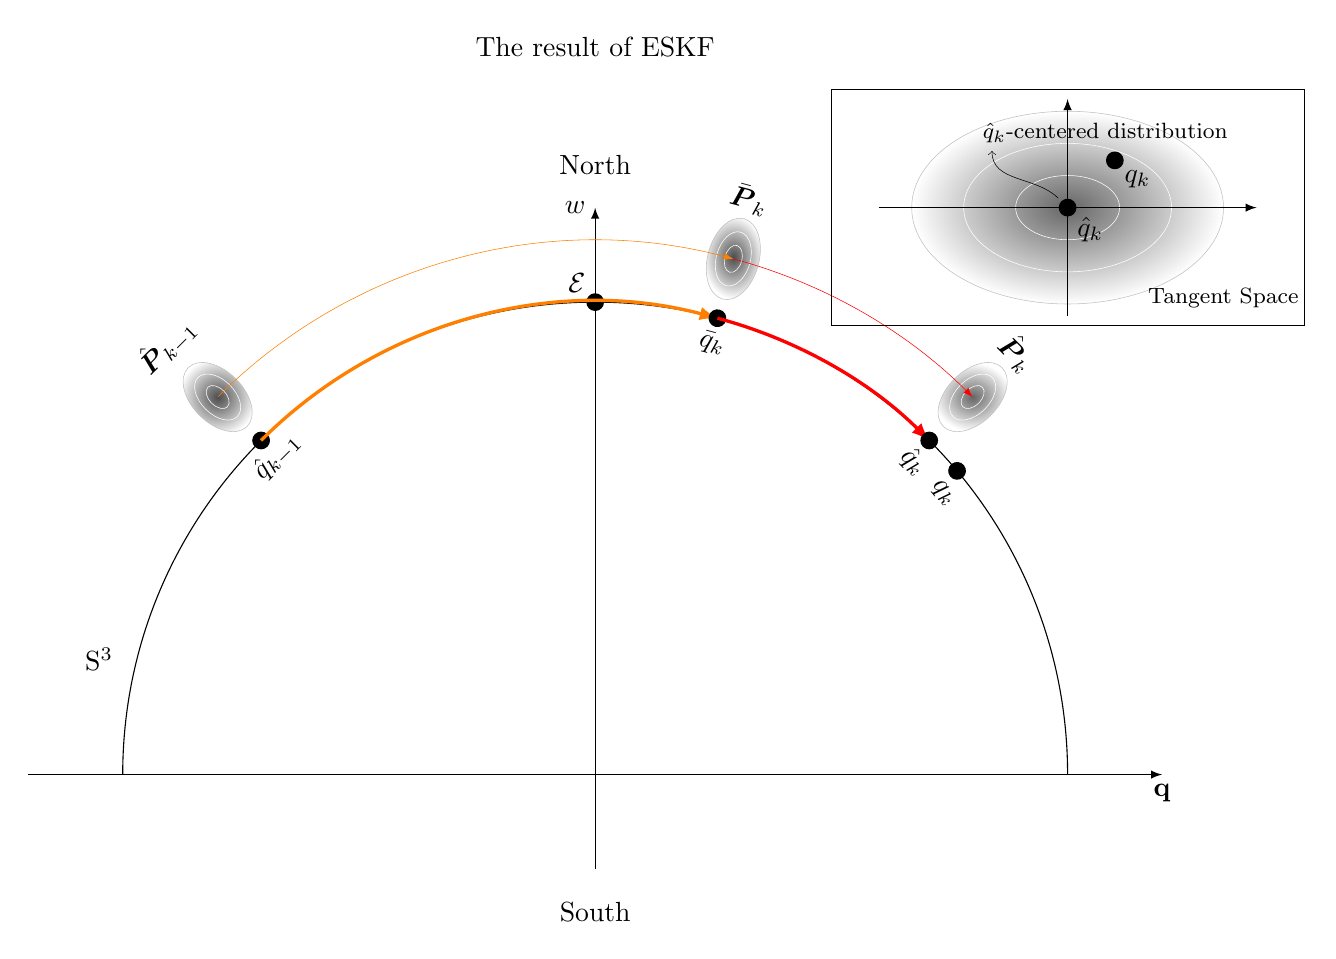
\begin{tikzpicture}[scale=6]

% Draw x and y axis lines
\draw [->,>=latex] (-1.2,0) -- (1.2,0) node [below] {$\mathbf{q}$};
\draw [->,>=latex] (0,-0.2) -- (0,1.2) node [left] {$w$};
\node [above] at (0, 1.25) {North};
\node [below] at (0,-0.25) {South};
\node[above left] at (-1.0,0.2) {$\mathrm{S}^{3}$};
\node[above] at (0.0,1.5) {The result of ESKF};

% Draw a arc at the origin of radius 1
\draw (1,0) arc (000:180:1);
\filldraw[black] (0,1) circle (0.5pt) node[above left ] {$\mathcal{E}$} ;

\begin{scope} [rotate=45]

\filldraw[black] (0.0,1.0) circle (0.5pt) node[below, rotate=45 ] {$\hat{q}_{k-1}$} ;

\begin{scope} [shift={(0.0, 1.13)}, scale=0.08]

% FIXME: 程序有BUG,旋转之后灰度边缘不对。
\draw [very thin, lightgray, inner color=black!70, outer color=black!0] (0,0) ellipse (0.68 and 1.1);
\draw [very thin, lightgray!0] (0,0) ellipse (0.68/3*2 and 1.1/3*2); % \sigma = +-2
\draw [very thin, lightgray!0] (0,0) ellipse (0.68/3   and 1.1/3  ); % \sigma = +-1

\node[above, rotate=45] at (0.0,1.21) {$\hat{\boldsymbol{P}}_{k-1}$};

\end{scope}

\draw [->,>=latex] [very thick, orange] (0,1) arc (90:30:1);

\end{scope}

\begin{scope} [rotate=-15]

\filldraw[black] (0.0,1.0) circle (0.5pt) node[below=2pt, rotate=-15 ] {$\bar{q}_{k}$} ;

\draw [->,>=latex] [very thick, red] (0,1) arc (90:60:1);

\begin{scope} [shift={(0.0, 1.13)}, scale=0.08]

% FIXME: 程序有BUG,旋转之后灰度边缘不对。
\draw [very thin, lightgray, inner color=black!70, outer color=black!0] (0,0) ellipse (0.68 and 1.1);
\draw [very thin, lightgray!0] (0,0) ellipse (0.68/3*2 and 1.1/3*2); % \sigma = +-2
\draw [very thin, lightgray!0] (0,0) ellipse (0.68/3   and 1.1/3  ); % \sigma = +-1

\end{scope}

\node[above, rotate=-15] at (0.0,1.21) {$\bar{\boldsymbol{P}}_{k}$};


\end{scope}

\begin{scope} [rotate=-45]

\filldraw[black] (0.0,1.0) circle (0.5pt) node[below=2pt, rotate=-45 ] {$\hat{q}_{k}$} ;

\begin{scope} [shift={(0.0, 1.13)}, scale=0.08]

% FIXME: 程序有BUG,旋转之后灰度边缘不对。
\draw [very thin, lightgray, inner color=black!60, outer color=black!0] (0,0) ellipse (0.68 and 1.1);
\draw [very thin, lightgray!0] (0,0) ellipse (0.68/3*2 and 1.1/3*2); % \sigma = +-2
\draw [very thin, lightgray!0] (0,0) ellipse (0.68/3   and 1.1/3  ); % \sigma = +-1

\end{scope}

\node[above, rotate=-45] at (0.0,1.21) {$\hat{\boldsymbol{P}}_{k}$};

\end{scope}

\begin{scope} [rotate=45]

\draw [->,>=latex] [very thin , orange] (0,1.13) arc (90:30:1.13);

\end{scope}

\begin{scope} [rotate=-15]

\draw [->,>=latex] [very thin , red] (0,1.13) arc (90:60:1.13);

\end{scope}

\begin{scope} [rotate=-50]

\filldraw[black] (0.0,1.0) circle (0.5pt) node[below=4pt, rotate=-50 ] {$q_{k}$} ;

\end{scope}

\begin{scope} [shift={(1.0, 1.2)}]

\draw [very thin] (-0.5,-0.25) rectangle (0.5,0.25);

\begin{scope} [scale=0.30]

% FIXME: 程序有BUG,旋转之后灰度边缘不对。
\draw [very thin, lightgray, inner color=black!60, outer color=black!0] (0,0) ellipse (1.1 and 0.68);
\draw [very thin, lightgray!0] (0,0) ellipse (1.1/3*2 and 0.68/3*2); % \sigma = +-2
\draw [very thin, lightgray!0] (0,0) ellipse (1.1/3   and 0.68/3  ); % \sigma = +-1

\end{scope}

\draw [->,>=latex] (-0.4, 0.00) -- ( 0.4, 0.00) ;
\draw [->,>=latex] ( 0.0,-0.23) -- ( 0.0, 0.23) ;

\filldraw[black] ( 0.0, 0.0) circle (0.5pt) node [below right] {$\hat{q}_{k}$};
\filldraw[black] ( 0.1, 0.1) circle (0.5pt) node [below right] {${q}_{k}$};

\node [below right] at (-0.20, 0.20) {\footnotesize $\hat{q}_{k}$-centered distribution};
\node [below right] at ( 0.15,-0.15) {\footnotesize Tangent Space};

\draw [very thin, ->] (-0.02, 0.02) to [out=135,in=-90] (-0.16, 0.12) ;

\end{scope}

\end{tikzpicture}

\end{document}

